%% Towards a Cartography of Datacentering
%% Research Policy 11th ECR Conference ,	extperiodcentered, 27 April 2026 ,	extperiodcentered, 14:27 BST
%% Theme: Metropolis + IBM Plex Sans (Carbon B&W)

\documentclass[aspectratio=169,11pt]{beamer}
\usetheme{metropolis}

\usepackage[sfdefault,light]{plex-sans}
\usepackage{plex-mono}
\renewcommand{\familydefault}{\sfdefault}
\usepackage{microtype}
\usepackage{booktabs}
\usepackage{tabularx}
\usepackage{array}
\usepackage{tikz}
\usepackage{graphicx}
\usepackage{fontawesome5}
\usepackage{colortbl}
\usepackage{xcolor}
\usepackage{textcomp}
\usetikzlibrary{arrows.meta,positioning,shapes.geometric,fit,backgrounds}

%% B&W Carbon palette
\definecolor{dcblue}{RGB}{22,22,22}
\definecolor{dcaccent}{RGB}{22,22,22}
\definecolor{dclightblue}{RGB}{218,218,218}
\definecolor{dcgray}{RGB}{110,110,110}
\definecolor{dchighlight}{RGB}{192,80,77}

\setbeamercolor{frametitle}{bg=black!88,fg=white}
\setbeamercolor{progress bar}{fg=black!55}
\setbeamercolor{alerted text}{fg=dchighlight}
\setbeamercolor{normal text}{fg=black!88,bg=white}
\setbeamercolor{background canvas}{bg=white}
\setbeamerfont{alerted text}{series=\bfseries}
\setbeamerfont{frametitle}{size=\normalsize,series=\bfseries}
\setbeamerfont{title}{size=\large,series=\bfseries}
\setbeamerfont{subtitle}{size=\normalsize,series=\mdseries}
\setbeamerfont{institute}{size=\footnotesize,series=\mdseries}
\setbeamerfont{date}{size=\footnotesize,series=\mdseries}
\setbeamerfont{block title}{size=\small,series=\bfseries}

\setbeamersize{text margin left=6mm, text margin right=6mm}
\hfuzz=6pt

\newcommand{\icon}[1]{\textcolor{dcblue}{\faIcon{#1}}\enspace}
\newcommand{\iconfull}[2]{\textcolor{#1}{\faIcon{#2}}}
\newcommand{\hl}[1]{\textcolor{dchighlight}{\textbf{#1}}}

\title{Towards a Cartography of Datacentering}
\subtitle{A Multimodal Research Agenda for Innovation Studies}
\author{Babajide Alamu Owoyele}
\institute{DRIFT, Erasmus University Rotterdam \textbar\ Radboud University}
\date{Research Policy 11th ECR Conference \textbar\ 27 April 2026}

\setbeameroption{hide notes}

%% ==================================================================
\begin{document}

%% ------------------------------------------------------------------
%% SLIDE 1 — Title  0:15
\begin{frame}[shrink=4]
\titlepage
\end{frame}
\note{I'm proposing a methodological cartography for studying data-center infrastructure as a contested innovation arena. Ten minutes.}

%% ------------------------------------------------------------------
%% SLIDE 2 — Empirical Moment  0:45
\begin{frame}{\iconfull{dcblue}{chart-bar}\enspace The Empirical Moment}
\begin{columns}[T]
\begin{column}{0.46\textwidth}
  \vspace{0.3em}
  \begin{tabular}{@{}lr@{}}
    \toprule
    \textbf{Metric} & \textbf{Value} \\
    \midrule
    Hyperscaler capex 2026   & \textbf{\$750B} \\
    DC electricity 2025      & 485~TWh (+17\%) \\
    AI-specific growth       & +50\% YoY \\
    Hyperscaler share 2031   & 67\% of all DC \\
    \bottomrule
  \end{tabular}
  \vspace{0.5em}

  \scriptsize\textcolor{dcgray}{CreditSights Feb 2026; IEA Energy \& AI April 2026;
  Synergy Research Group}
\end{column}
\begin{column}{0.50\textwidth}
  \vspace{0.5em}
  \large\textit{``The largest concentrated\\
  infrastructure build of our\\
  lifetimes — happening now.''}\\[0.6em]
  \normalsize
  Not a future scenario.\\
  Not a policy proposal.\\[0.4em]
  \hl{An arena in formation.}
\end{column}
\end{columns}
\note{Lead with the dollar number. Point at the table. Hyperscaler capex is the largest concentrated infrastructure build of our lifetimes. Three years.}
\end{frame}

%% ------------------------------------------------------------------
%% SLIDE 3 — Why Now  0:45
\begin{frame}{\iconfull{dcblue}{fire}\enspace Why Now? The Contested Arena}
\begin{columns}[T]
\begin{column}{0.52\textwidth}
  \footnotesize
  \begin{itemize}\setlength\itemsep{0.4em}
    \item \textbf{Stargate:} \$500B / ${\sim}$7\,GW; OpenAI + Oracle + SoftBank
    \item \textbf{PJM electricity:} capacity prices \hl{+833\%} in one year
    \item \textbf{Maine:} first US statewide moratorium, April 2026
    \item \textbf{Loudoun Co.:} eliminates by-right DC, March 2025
    \item \textbf{DeepSeek V4-Pro:} re-opens Jevons paradox debate
  \end{itemize}
\end{column}
\begin{column}{0.44\textwidth}
  \vspace{0.4em}
  \begin{block}{}
    \footnotesize
    \hl{37,552 DCD articles}\\[2pt]
    2008--2026, headline + intro\\[2pt]
    \textbf{1,073 contestation events}\\[2pt]
    Peak contestation: 2025\\[4pt]
    \textcolor{dcgray}{\scriptsize Trade press = primary event record before academic literature}
  \end{block}
\end{column}
\end{columns}
\note{The arena is contested right now. Maine moratorium is April 2026 — last month. We have 37,552 articles, 1,073 contestation events.}
\end{frame}

%% ------------------------------------------------------------------
%% SLIDE 4 — The Gap  0:45
\begin{frame}{\iconfull{dcblue}{search}\enspace The Gap in Innovation Studies}
\begin{columns}[T]
\begin{column}{0.48\textwidth}
  \small\textbf{RP canon covers:}\\[0.3em]
  \footnotesize
  Platforms (Gawer 2014)\\
  GPTs (Brynjolfsson)\\
  Sectoral systems (Malerba)\\
  Transitions (Geels)\\[0.5em]
  \small\textbf{Critical DC studies exists:}\\[0.3em]
  \footnotesize
  \textit{Big Data \& Society}, \textit{Convergence}\\
  Edwards et al.\ 2025; Monstadt 2025\\
  — but outside RP's canon
\end{column}
\begin{column}{0.48\textwidth}
  \vspace{0.3em}
  \begin{tikzpicture}[font=\footnotesize]
    \node[draw=dchighlight,rounded corners=2pt,
          inner sep=8pt,text width=4.5cm,fill=black!3] {
      \textbf{Missing:}\\[4pt]
      Integrative framework for the\\
      \textit{infrastructural + methodological}\\
      turn in AI-era innovation studies\\[5pt]
      No unified approach to:\\
      \textbullet\ mapping contested arenas\\
      \textbullet\ surfacing implicated actors\\
      \textbullet\ operationalizing multimodal evidence
    };
  \end{tikzpicture}
\end{column}
\end{columns}
\note{RP has the tools — arenas, transitions, sectoral systems. Critical data-center studies exists but outside RP. Nobody has bridged them. That's the gap.}
\end{frame}

%% ------------------------------------------------------------------
%% SLIDE 5 — Theory: Arenas  0:50
\begin{frame}{\iconfull{dcblue}{users}\enspace Theory: Arenas of Development}
\begin{columns}[T]
\begin{column}{0.52\textwidth}
  \small\textbf{Jørgensen (2012) — \textit{Research Policy}}\\[0.3em]
  \footnotesize
  Flat ontology. Start from \textit{actor\\
  constellations} and their collective\\
  engagement — not structural tiers.\\[0.4em]
  \textbf{Negotiation} is the fundamental process.\\[0.4em]
  Allows political, social, environmental\\
  spheres simultaneously.\\[0.5em]
  \small\textbf{+ Clarke (2005): situational maps}\\[0.3em]
  \footnotesize
  Implicated actors: silenced (communities,\\
  visa workers) + constructed but absent\\
  (``the consumer'', ``future generations'')
\end{column}
\begin{column}{0.44\textwidth}
  \vspace{0.3em}
  \footnotesize\textbf{The datacentering arena:}\\[0.4em]
  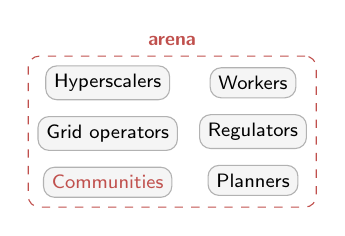
\begin{tikzpicture}[font=\scriptsize,node distance=0.2cm,
    actor/.style={draw=black!30,rounded corners,inner sep=3pt,fill=black!4}]
    \node[actor] (h)  {Hyperscalers};
    \node[actor,below=of h] (g) {Grid operators};
    \node[actor,below=of g] (c) {\textcolor{dchighlight}{Communities}};
    \node[actor,right=0.5cm of h] (w)  {Workers};
    \node[actor,below=of w] (r)  {Regulators};
    \node[actor,below=of r] (p)  {Planners};
    \node[draw=dchighlight,dashed,rounded corners,
          fit=(h)(g)(c)(w)(r)(p),
          label=above:{\textcolor{dchighlight}{\textbf{arena}}}]{};
  \end{tikzpicture}
  \vspace{0.3em}

  \footnotesize Co-constitutive.\\
  Not hierarchically ordered.
\end{column}
\end{columns}
\note{Arenas not levels. Flat ontology. Negotiation is the fundamental process. Jørgensen is in RP 2012 — this is your canon. Clarke gives us implicated actors — who is excluded from the negotiation.}
\end{frame}

%% ------------------------------------------------------------------
%% SLIDE 6 — Theory: Marres + CITC  0:50
\begin{frame}{\iconfull{dcblue}{network-wired}\enspace Theory: Issue Mapping + CITC}
\begin{columns}[T]
\begin{column}{0.50\textwidth}
  \small\textbf{Marres (2015) — \textit{ST\&HV}}\\[0.3em]
  \footnotesize
  Issue mapping via digital traces.\\
  Trade press, hyperlinks, hashtags as\\
  empirical window into issue formation.\\[0.5em]
  \small\textbf{Berente et al.\ (2019); Miranda et al.\ (2022)}\\[0.2em]
  \small\textbf{Computationally Intensive Theory Construction}\\[0.3em]
  \footnotesize
  Sampling $\to$ synchronic $\to$ diachronic\\
  $\to$ \textbf{lexical framing}\\[0.3em]
  Patterns become contributions \textit{only}\\
  once situated in scholarly discourse.
\end{column}
\begin{column}{0.46\textwidth}
  \vspace{0.6em}
  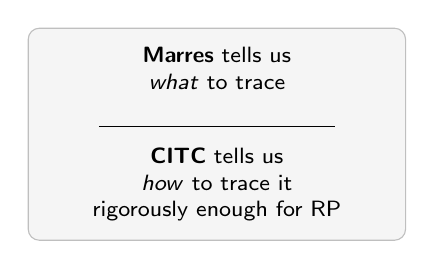
\begin{tikzpicture}[font=\footnotesize]
    \node[draw=black!25,rounded corners,fill=black!4,
          inner sep=7pt,text width=4.3cm,align=center] {
      \textbf{Marres} tells us\\
      \textit{what} to trace\\[4pt]
      \rule{3cm}{0.3pt}\\[4pt]
      \textbf{CITC} tells us\\
      \textit{how} to trace it\\
      rigorously enough for RP
    };
  \end{tikzpicture}
  \vspace{0.4em}

  \footnotesize\textcolor{dcgray}{Prevents atheoretical\\
  pattern-mining.}
\end{column}
\end{columns}
\note{One sentence: Marres tells us what to trace. CITC tells us how to trace it rigorously enough to make a theoretical contribution. That's the methodological spine.}
\end{frame}

%% ------------------------------------------------------------------
%% SLIDE 7 — Data: DCD EDA  (0:45)
\begin{frame}{\iconfull{dcblue}{chart-line}\enspace The Arena in Data}
\begin{columns}[T]
\begin{column}{0.50\textwidth}
  \includegraphics[width=\textwidth,height=0.65\textheight,keepaspectratio]%
    {../figures/dcd_eda_timeline}
\end{column}
\begin{column}{0.46\textwidth}
  \includegraphics[width=\textwidth,height=0.65\textheight,keepaspectratio]%
    {../figures/dcd_eda_geography}
\end{column}
\end{columns}
\vspace{0.15em}
\scriptsize\textcolor{dcgray}{%
  37,552 articles ,	extperiodcentered, 1,073 contestation events ,	extperiodcentered, peak 2025.
  \textbf{Headlines + intro text only} — full articles via screenshot/OCR pipeline.
  More coming.}
\note{This is from the real corpus. 37,552 articles, 2008 to 2026. Peak contestation in 2025. Maine statewide moratorium is in this data. The arena is visible in the trade press record.}
\end{frame}

%% ------------------------------------------------------------------
%% SLIDE 8 — Register analysis  (0:45)
\begin{frame}{\iconfull{dcblue}{font}\enspace The Register Shift}
\begin{columns}[T]
\begin{column}{0.50\textwidth}
  \includegraphics[width=\textwidth,height=0.65\textheight,keepaspectratio]%
    {../figures/register_contrast}
\end{column}
\begin{column}{0.46\textwidth}
  \vspace{0.4em}
  \small\textbf{Matthiessen (2015) registerial\\
  cartography — verb process types}\\[0.4em]
  \footnotesize
  \begin{tabular}{@{}lrr@{}}
    \toprule
    Type & Contest & Non \\
    \midrule
    Behavioral & 23.1\% & 1.6\% \\
    Enabling   & 16.5\% & 3.1\% \\
    Material   & 33.7\% & 66.8\% \\
    \bottomrule
  \end{tabular}
  \vspace{0.4em}

  \footnotesize
  \textit{Doing} $\to$ \textit{governing + contesting}\\[0.3em]
  \hl{The governance gap visible\\
  in the verb register.}\\[0.3em]
  \textcolor{dcgray}{\scriptsize Headlines + intros only.}
\end{column}
\end{columns}
\note{The register shift IS the governance gap made linguistic. Behavioral verbs up 21.5\%. Enabling verbs up 13.4\%. Material verbs drop 33\%. The arena shifts from building to governing and contesting.}
\end{frame}

%% ------------------------------------------------------------------
%% SLIDE 9 — city2graph  (0:45)
\begin{frame}{\iconfull{dcblue}{city}\enspace City2Graph: Urban Embeddedness}
\begin{columns}[T]
\begin{column}{0.50\textwidth}
  \includegraphics[width=\textwidth,height=0.68\textheight,keepaspectratio]%
    {../figures/wp3_urban_graphs_map}
\end{column}
\begin{column}{0.46\textwidth}
  \vspace{0.4em}
  \small\textbf{From corpus cities $\to$ urban graphs}\\[0.3em]
  \footnotesize
  GLiNER NER extracts city names\\
  $\to$ city2graph pulls Overture Maps\\
  $\to$ graph: DC node $\leftrightarrow$ power,\\
  \hspace{1.2em}residential, commercial\\[0.4em]
  \begin{tabular}{@{}lrr@{}}
    & Res.\ zones & Power \\
    \midrule
    Ashburn  & 1  & 36 \\
    Amsterdam & 61 & 2  \\
    Dublin   & 361 & 6  \\
  \end{tabular}
  \vspace{0.4em}

  \footnotesize\hl{Spatial embeddedness\\
  determines governance\\
  counterparty availability.}
\end{column}
\end{columns}
\note{The structural difference — Ashburn isolated, Amsterdam embedded — is not just a planning story. It's a spatial story. The urban graph makes it systematic.}
\end{frame}

%% ------------------------------------------------------------------
%% SLIDE 10 — Three research agendas  (1:30 — 0:30 each)
\begin{frame}[shrink=3]{\iconfull{dcblue}{map}\enspace Three Research Agendas}
\vspace{-0.1em}
{\footnotesize\setlength{\tabcolsep}{4pt}
\begin{tabularx}{\linewidth}{@{}>{\bfseries\raggedright}p{2.6cm}XX@{}}
\toprule
\rowcolor{black!88}
\textcolor{white}{\textbf{Agenda}} &
\textcolor{white}{\textbf{Central question}} &
\textcolor{white}{\textbf{Cases}} \\
\midrule
Regional Innovation Systems &
How do hyperscale clusters reshape local productivity, labour, energy, property? &
Loudoun (US), Lule\aa\ (SE), Dublin (IE), Hyderabad (IN) \\
\rowcolor{black!8}
Sectoral Transformation &
How does hyperscaler vertical integration reshape sectoral systems and startup access? &
AWS, Google, Meta, Microsoft platform dependency \\
Policy Sovereignty \& Energy &
What policy mix sustains sovereign compute without fossil lock-in or geopolitical dependency? &
UK AI Growth Zones, EU AI Factories, France, Saudi HUMAIN, UAE Stargate \\
\bottomrule
\end{tabularx}}
\vspace{0.2em}
\footnotesize\textcolor{dcgray}{Each agenda operationalized via the CITC cycle (Berente et al.\ 2019): sampling $\to$ synchronic $\to$ diachronic $\to$ lexical framing.}
\note{Three agendas, 30 seconds each. Question, cases — don't dwell. These are programs the cartography enables.}
\end{frame}

%% ------------------------------------------------------------------
%% SLIDE 11 — Open cartography  (0:30)
\begin{frame}{\iconfull{dcblue}{folder-open}\enspace Building the Cartography Together}
\begin{columns}[T]
\begin{column}{0.52\textwidth}
  \small\icon{share-alt}\textbf{Why open is theoretical necessity}\\[0.2em]
  \footnotesize
  CAS-like phenomena are too distributed,\\
  too opaque for any single team.\\[0.4em]
  \small\icon{tools}\textbf{What we share}
  \begin{itemize}\footnotesize
    \item Facility index (CC BY 4.0)
    \item NLP / CV / network pipelines (MIT)
    \item DCD contestation corpus
    \item Register + NER analysis scripts
    \item \texttt{github.com/babajideowoyele/}\\\texttt{datacentering-cartography}
  \end{itemize}
\end{column}
\begin{column}{0.44\textwidth}
  \vspace{0.2em}
  \small\icon{hands-helping}\textbf{Concrete asks}
  \begin{itemize}\footnotesize
    \item Local planning records + disputes
    \item Non-English corpus (NL, DE, FR, IE)
    \item Company registry / REIT data access
    \item Replication in other jurisdictions
    \item Methodological critique
  \end{itemize}
  \vspace{0.5em}
  \begin{center}
    \small\textit{``What would innovation studies\\
    look like if we treated data\\
    infrastructure as \alert{foundational}\\
    rather than peripheral?''}
  \end{center}
\end{column}
\end{columns}
\note{The distributed observatory is the methodological response to the distributed object. Come build it with us.}
\end{frame}

%% ==================================================================
\appendix

\begin{frame}[noframenumbering]{\faIcon{question-circle}\enspace Q: Isn't this STS dressed up as innovation studies?}
\footnotesize
\textbf{Live:} ``Fair concern — I'm using Jørgensen and Marres specifically because they bridge to RP and \textit{ST\&HV}, not importing critical theory wholesale.''\\[0.5em]
The methodological spine — CITC (Berente, Seidel \& Safadi 2019; Miranda et al.\ 2022) — comes from \textit{MIS Quarterly} and \textit{ISR}, not from STS. The agenda is testable, not hermeneutic.
\end{frame}

\begin{frame}[noframenumbering]{\faIcon{question-circle}\enspace Q: Where's the empirical contribution?}
\footnotesize
\textbf{Live:} ``The ECR paper is the agenda. The corpus analysis is the first empirical instantiation.''\\[0.5em]
From 37,552 DCD articles:\\[0.3em]
\begin{tabular}{@{}lll@{}}
\toprule
\textbf{Analysis} & \textbf{Status} & \textbf{Finding} \\
\midrule
EDA geography     & Complete  & US/Europe split; peak 2025 \\
Register analysis & Complete  & Behavioral +21.5\%, enabling +13.4\% \\
BERTopic topics   & Running   & Full corpus topic clusters \\
city2graph        & Seed run  & 3 cities; scales via GLiNER NER \\
\bottomrule
\end{tabular}\\[0.3em]
\textcolor{dcgray}{\textit{Analysis on headlines + intros. Full article text: screenshot/OCR pipeline coming.}}
\end{frame}

\begin{frame}[noframenumbering]{\faIcon{question-circle}\enspace Q: Why Loudoun, Luleå, Dublin, Hyderabad?}
\footnotesize
\textbf{Variation on three dimensions:}\\[0.4em]
\begin{tabular}{@{}llll@{}}
\toprule
\textbf{Case} & \textbf{Regulatory} & \textbf{Energy} & \textbf{Trajectory} \\
\midrule
Loudoun    & Common law / NIMBY  & Gas + solar  & Mature US cluster \\
Lule\aa    & Swedish planning    & 98\% hydro   & Renewable-led \\
Dublin     & Irish planning      & Mixed        & FDI platform \\
Hyderabad  & Indian regulatory   & Expanding    & Emerging hub \\
\bottomrule
\end{tabular}
\end{frame}

\begin{frame}[noframenumbering]{\faIcon{question-circle}\enspace Q: What are the register verb families?}
\footnotesize
Following Matthiessen (2015) Hallidayan process types — applied to DCD headlines + intros:\\[0.4em]
\begin{tabular}{@{}lll@{}}
\toprule
\textbf{Process type} & \textbf{Field of activity} & \textbf{Top verbs in corpus} \\
\midrule
Material    & Doing / building      & secures, builds, launches, withdraws, rejects \\
Verbal      & Reporting             & says, announces, claims, warns, demands \\
Mental      & Exploring / sharing   & opposes, concerns, challenges, supports \\
Relational  & Expounding            & is, becomes, remains, includes \\
Enabling    & Enabling              & bans, permits, rezones, mandates, regulates \\
Behavioral  & Contesting            & protests, campaigns, sues, appeals, petitions \\
\bottomrule
\end{tabular}\\[0.3em]
\textcolor{dcgray}{\textit{Contestation = shift from material/relational to behavioral/enabling.}}
\end{frame}

\begin{frame}[noframenumbering]{\faIcon{question-circle}\enspace Q: Why CITC and not CSS more broadly?}
\footnotesize
CITC's lexical-framing requirement is what makes the output theoretical, not just descriptive.\\[0.5em]
That's the discipline that protects against the most common reviewer objection:\\[0.3em]
\begin{quote}
  ``This is interesting, but what's the theoretical contribution?''
\end{quote}
\vspace{0.3em}
CITC explicitly distinguishes patterns from contributions. The test for RP.
\end{frame}

\end{document}
